\begin{comment}

\subsection{PARTICLE IMAGE VELOCIMETRY}

$PIV$ is a technique to determine the  velocity field of objects from a stream of images\cite{Bastiaans}.
The result of the $PIV$ is given as a vector field, showing for each particle, direction, sense and intensity of velocity. 
Moreover, the $PIV$ can be used for track different objects in the same image.
For this purpose, the $PIV$ technique divides a frame, by example the frame 1, in many possibles regions where targets can be found; 
to this purpose, each region of frame 1 and 2 are correlated using comparative method, 
so that a vector or a field of vector is generated 
starting of initial point till final point. Thus, we have displacement and the acquisition time between frames, 
so that applying derivate concepts it is possible to estimate the relative velocity.

\begin{figure}[H]
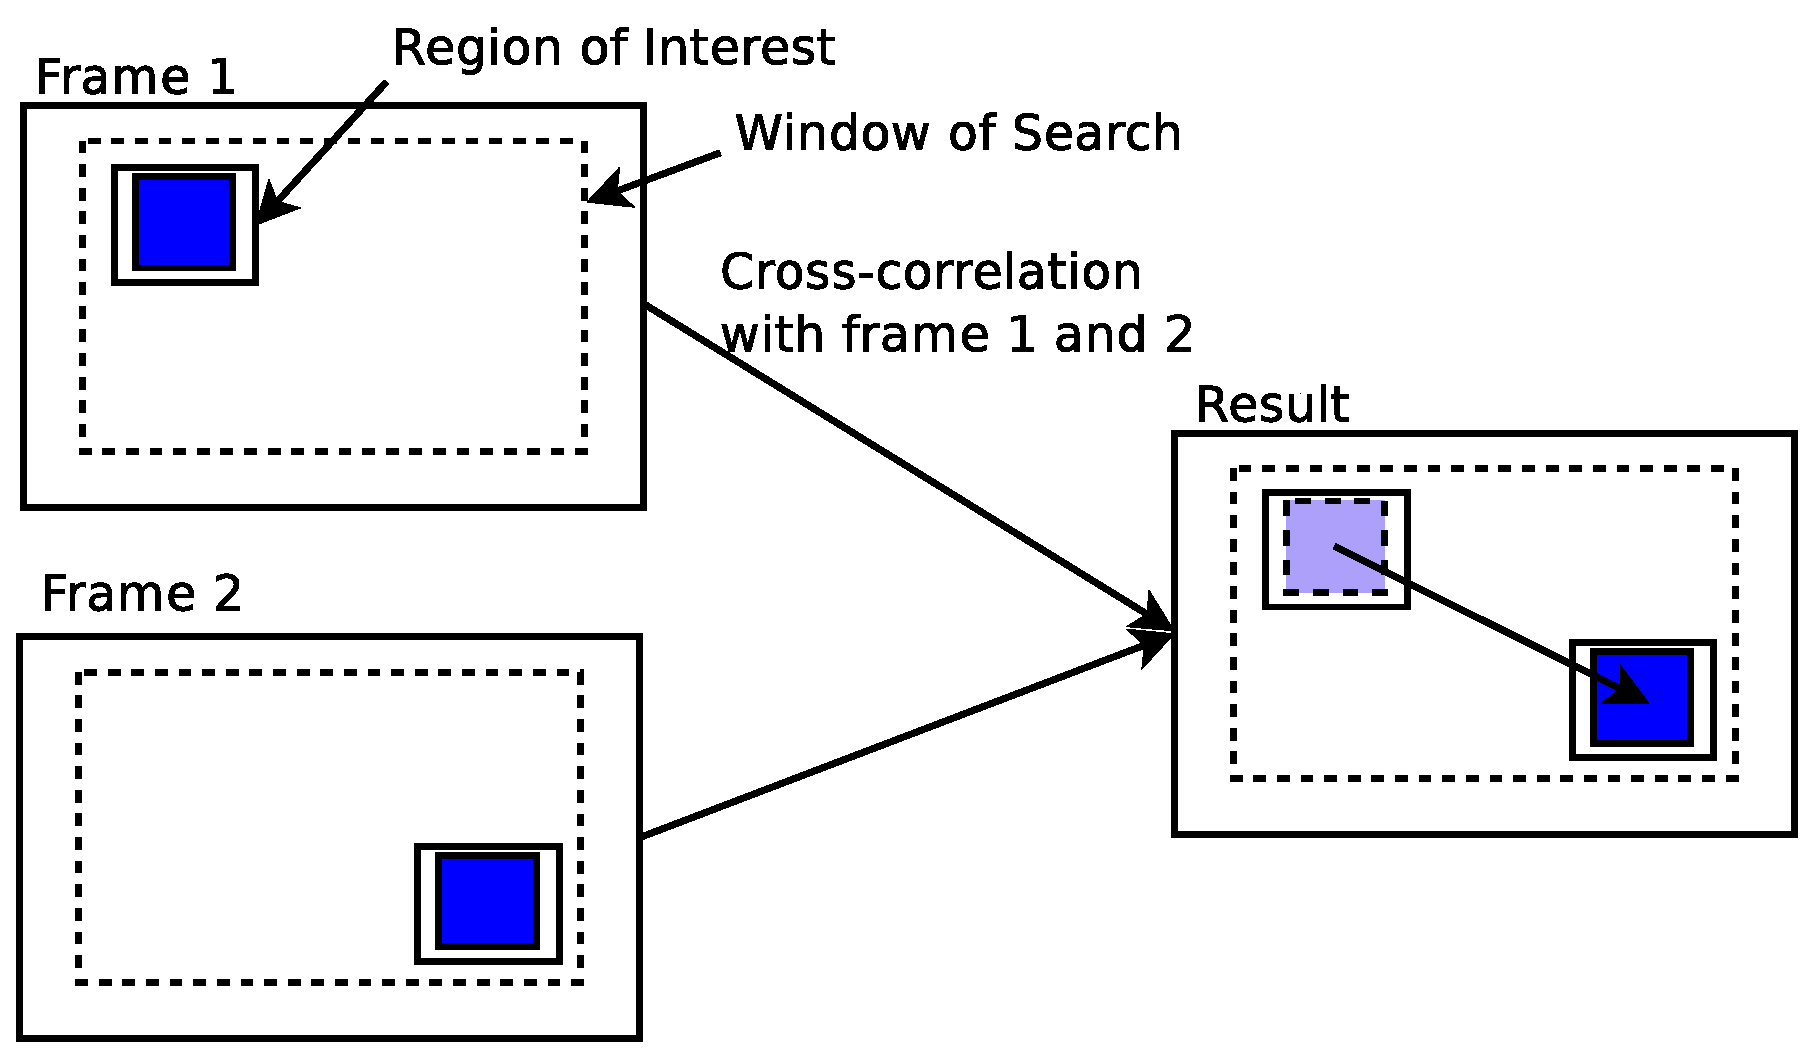
\includegraphics[width=\columnwidth]{images/explanationPIV.eps}
\caption{The PIV operation comparing two frames}
\label{fig:twoframes}
\end{figure}

The Fig. \ref{fig:twoframes} illustrates how $PIV$ works and demonstrates the relation between Region of Interest ($ROI$) and 
Window of Search ($WOS$). where $WOS$ is a region where the target will be searched and consequently $WOS$ must involve ROI. 
$WOS$ doesn't fill necessary whole image. If $WOS$ is large, we have an augment of computing but 
if $WOS$ is too small, target in high velocity has more chances to be lost. In our application, 
we determine $WOS$ from $1.5$ of $ROI$. For example, if ROI is $200\times300$ so we have WOS of $300\times450$. 
This consideration can be tuned by tests, by example considering environments with objects
of low velocity (permitted velocity in cities and roads).

\begin{figure}[H]
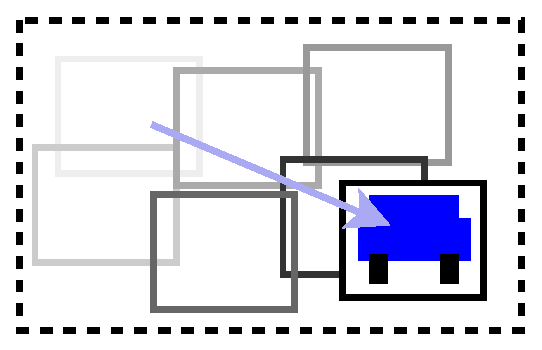
\includegraphics[width=\columnwidth]{images/WOSdivided.eps}
\caption{The $ROI$ is searched in the $ROI$ on windows of same dimensions. }
\label{fig:WOSdivided}
\end{figure}

$ROI$ is one of most important part of $PIV$, because it contains target. An Analysis Region ($AR$)
of same dimension of $ROI$ is displaced
along of whole $WOS$ in frame $2$, like showed in Fig. \ref{fig:WOSdivided}. Comparisons are done among regions between frames and are 
assigned values. 
When process finishes, the more height value refers the new place of $ROI$. It means that target displaced of a point in 
frame $1$ to another in frame $2$.

\end{comment}

%%%%%%%%%%%%%%%%%%%%%%%%%%%%%%%%%%%%%%%%%%%%%portugues%%%%%%%%%%%%%%%%%%%%%%%%%%%%%%%%%%%%%%%%%%%%%%%%%%%%%%%%%%%%%

\subsection{Velocimetria por Imagem de Partículas}

A Velocimetria por imagem de partículas (PIV, do inglês Particle Image Velocimetry) 
é um método óptico que permite a visualização e a análise do movimento de partículas em fluidos, no caso aplicado em imagens \cite{Bastiaans}.
O resultado do $PIV$ é dado por um campo vetorial que representa a direção, sentido e intensidade da velocidade de cada 
partícula. Além disso, pode ser usado para acompanhar objetos dentro de um fluxo de imagens sequenciais, obtidas por uma câmera por exemplo.

O $PIV$ divide a imagem em diferentes possíveis regiões de interesse, onde o objeto de interesse pode ser encontrado. 
A região que contém o objeto de 
interesse é correlacionada com a próxima imagem do fluxo, no caso deste exemplo, a imagem 2. 
Após ser encontrado sua correspondente, um vetor é traçado do ponto inicial
até a região encontrada. Assim, evidencia-se um deslocamento entre uma imagem e outra em seguida, aplicando-se  a derivada 
é possível obter a  estimativa da velocidade relativa.

\begin{figure}[H]
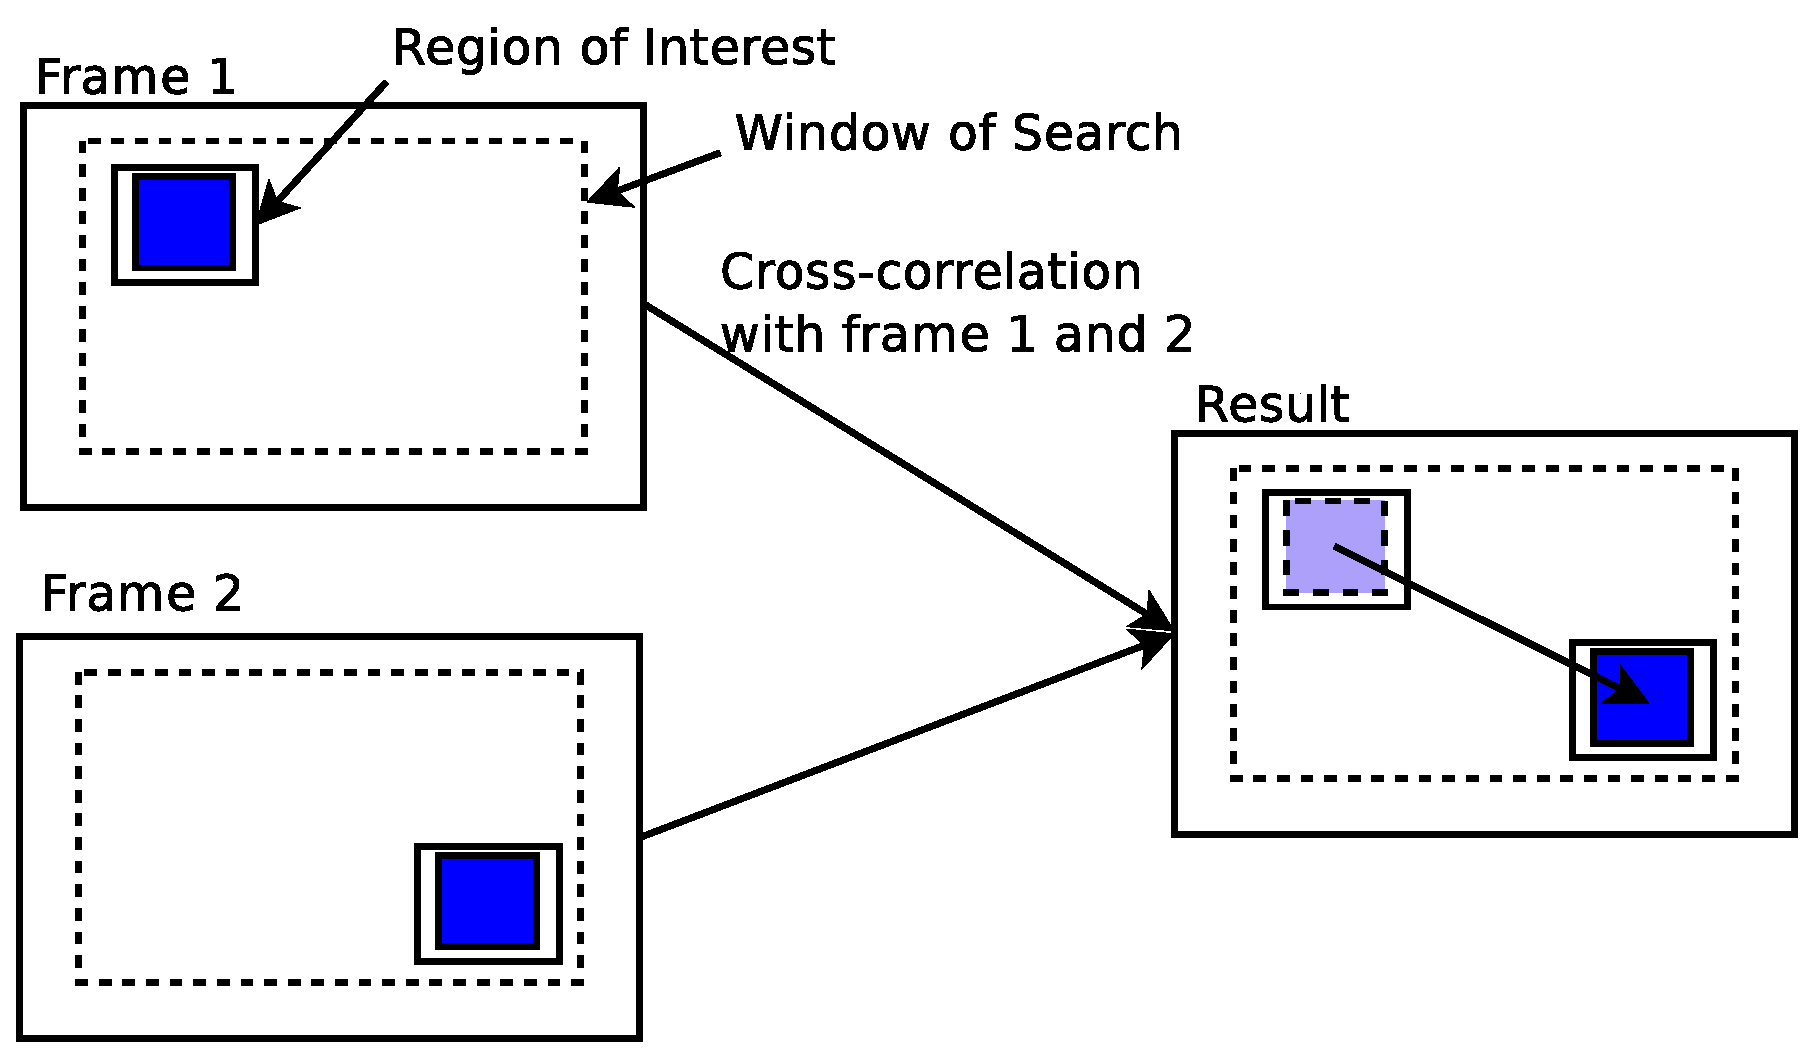
\includegraphics[width=\columnwidth]{images/explanationPIV.eps}
\caption{Funcionamento do $PIV$, comparando duas imagens.}
\label{fig:twoframes}
\end{figure}

A Figura \ref{fig:twoframes} ilustra como o $PIV$ funciona, 
destaque para a relação entre a região de interesse ou $ROI$ (do inglês ``Region of Interesting'') e 
a janela de busca ou $WOS$  (do inglês ``Windowm of Search''). 
A $WOS$ é a região onde o objeto de interesse pode ser encontrado,
neste artigo esta é selecionada como sendo $1.5$ vesses o tamanho do $ROI$. 
Por exemplo, se o $ROI$ tem dimensão $200\times300$, então a $WOS$ terá $300\times450$.
Essa consideração foi tomada a partir dos testes que 
levavam em conta os \colorbox{red}{limites de velocidade permitidos em cidades e rodovias}.


\begin{figure}[H]
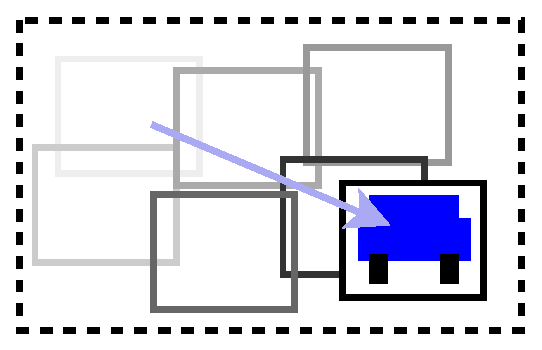
\includegraphics[width=\columnwidth]{images/WOSdivided.eps}
\caption{O $WOS$ é o espaço pelo qual o $ROI$ será procurado.}
\label{fig:WOSdivided}
\end{figure}

$ROI$ é uma das partes mais importantes do $PIV$, pois ele contém o objeto de interesse. Uma região de análise
($AR$) da mesma dimensão do $ROI$ é percorrida pelo $WOS$ na imagem 2, como mostrado na Figura \ref{fig:WOSdivided}.
As comparações usando $CCP$, são realizadas entre as regiões de ambas imagens e são 
calculados valores de correlação. Quando o processo termina, a posição da região com o maior valor
de correlação é a nova posição do objeto. Deste modo, traça-se um vetor do ponto inicial ($ROI$ na imagem 1) até o ponto final
($ROI$ na imagem 2).
